\renewcommand\thesubsection{\Alph{subsection}}
\numberwithin{equation}{subsection}
\numberwithin{figure}{subsection}
\section*{Appendices}
\addcontentsline{toc}{section}{Appendices}

\subsection{Discussion on angular momentum subspaces for different spins}
\label{app:angular-subspaces}

As we mentioned in the Section~\ref{sec:bg-the-quantu-state}, when dealing with many particle systems, the Hilbert space is represented by tensor product of the subspaces with a fixed spin.
So, the final dimension is the product of all single-particle dimensions which lead to an exponentially large Hilbert space.
In order to simplify many of the computations we work with, it is worth to note that some interesting structures arise from this kind of tensor product construction.

Let us name some basic assumptions with which the problem of adding angular momentum subspaces is simplified even further.
First of all, the single particle Hilbert space must be discrete and finite, hence it can be represented by a $d$-level system or qudit, where $d$ is the dimension of the single-particle system.
When $d$ equals two, we have the well known 2-level system or qubit.
The basis of such systems is composed by $d$ different eigenstates of the spin operator $j_z^{(n)}$, where $n$ denotes the Hilbert space in which the operator is defined.
We also assume that all parties have the same dimension $d$, so the total dimension is $d^N$.
The spin $j$ is defined as $j:=(d-1)/2$.
It is usual to use the single-particle angular momentum projector operator in the $z$-direction to completely characterize the basis
\be
  j_z^{(n)}\ket{m} = m \ket{m},
\ee
where $m = -j,-j+1,\dots,+j-1,+j$ and this way the necessary $d$ different pure states are defined.

In quantum information, the two eigenstates $\ket{-1/2}$ and $\ket{+1/2}$ of the 2-level systems, or qubits, are usually identified with $\ket{0}$ and $\ket{1}$ respectively, since the qubit case is the most studied case on which the dichotomized representation of classical \emph{bit}s, ones and zeros, is directly related with.
For qudits, particles whit $d$ levels, one can map directly the $m=-j,-j+1,\dots,+j-1,+j$ to $\tilde{m}=0,1,\dots,d-1$ in a similar way as for qubits, where $\tilde{m}$ is usual label used in the quantum information framework, whereas the $m$ gives directly the eigenvalue of the state when $j_z^{(n)}$ is applied.

A first approach to write a concise eigenbasis for the whole Hilbert space is to multiply by tensor product all the eigenstates of each single party.
This way, and permuting all the states from right to left, we construct a well defined basis as
\be
  \label{eq:app-eigenbasis-tensor-product}
  \begin{split}
    & \ket{-j,-j,\dots,-j,-j},\\
    & \ket{-j,-j,\dots,-j,-j+1},\\
    & \vdots \\
    & \ket{-j,-j,\dots,-j+1,-j},\\
    & \ket{-j,-j,\dots,-j+1,-j+1},\\
    & \vdots \\
    & \ket{+j,+j,\dots,+j,+j},
  \end{split}
\ee
where we have used the notation $\ket{m_1,m_2,\dots,m_{N-1},m_N}\equiv \ket{m_1}\otimes\ket{m_2}\dots\otimes\ket{m_N}$.
This basis is yet an eigenbasis of $J_z = \sum_{n} j_z^{(n)}$.
On the other hand, it is not an eigenbasis of the total angular momentum $\bs{J}^2 = J_x^2+J_y^2+J_z^2$, neither all the eigenstates are permutationally invariant, which is useful for dealing with symmetric subspaces.

We will explain shortly how to write a basis in which all members are eigenstates of the total angular momentum $\bs{J}^2$ as well as of the $J_z$ operator.
This is a usual procedure when adding angular momentum operators, see Ref.~\cite{Cohen-Tannoudji1977, Sakurai2010} for more details.
For that, we have the ladder $J_{\pm} := J_x \pm i J_y$ operators which increase or decrease the eigenvalue of the state when $J_z$ is applied without changing the eigenvalue for $\bs{J}^2$.
Therefore, if we start from $\ket{-j,-j,\dots,-j}$, which is an eigenstate of $\bs{J}^2$ with the maximal eigenvalue $Nj(Nj+1)$, and we apply $J_+$ subsequently we obtain all the states belonging to that subspace on which $\bs{J}^2$ is maximal.
We use the following notation for the maximal eigenvalue of the $\bs{J}^2$ operator
\be
  \label{eq:app-maximum-total-angular-momentum}
  \mathcal{J}_{Nj} \equiv Nj(Nj+1),
\ee
since it appears many times throughout the thesis.
Then, we use orthogonal states and we keep doing this until we have all the subspaces characterized.

Hence, the eigenstates are characterized with only three simple numbers $\ket{J,M,D}$ instead of Eq.~\eqref{eq:app-eigenbasis-tensor-product}.
First of all, we have the total angular momentum number $J$, where $J=0,1,\dots,Nj$ for this particular case in which we are adding together $N$ spin-$j$ particles (we also assume that if the spin number $j$ equals we have even number of particles for simplicity), and defined the eigenvalue of the $\bs{J}$ operator as $J(J+1)$.
Then, we have the quantum number of the angular momentum projection into the $z$-direction, $M=-J,-J+1,\dots,+J-1,+J$, which corresponds to the eigenvalue of the $J_z$ operator.
And finally, the degeneracy number of the $J$ subspaces, $D=1,2,\dots,D_J$, that is always one for the $J=Nj$ subspace and for the rest it depends in general in the number of particles as well as in the spin-number $j$.

We now show the definition of some of the most used states throughout this thesis.
For the spin-$\frac{1}{2}$ particles, i.e., qubits, several states appear.
For instance, the symmetric states, i.e., the states that interchanging any pair of particles remain the same, are all confined into the subspace where $J=\frac{N}{2}$ is maximal.
They can be constructed taking $n$ particles in the $\ket{-1/2}$ or $\ket{0}$ state, depending on the framework, and $N-n$ in the $\ket{+1/2}$ or $\ket{1}$ state and symmetrizing them as
\be
  \label{eq:ap-symmetric-states-qubits}
  \ket{J=N/2, M} \equiv \binom{N}{N/2+M}^{-1/2}\sum_k \mathcal{P}_k(\ket{0}^{\otimes n}\otimes\ket{1}^{\otimes{N-n}}),
\ee
where the sum is over all possible different permutations of the state denoted by $\mathcal{P}_k$ and $M=N/2-n$.
Note that the Dicke states, are named after R. H. Dicke, who used them to explain the coherent superradiance effect \cite{Dicke1954}.
If we consider two modes corresponding to the two states, then Eq.~\eqref{eq:ap-symmetric-states-qubits} is equivalent to the twin Fock state for a constant particle number.
Therefore apart from Eq.~\eqref{eq:ap-symmetric-states-qubits}, we use the following notation for these states
\be
  \ket{\dicke{N, n}} \equiv \ket{J=N/2, M=N/2-n}=\binom{N}{N-n}^{-1/2}\sum_k \mathcal{P}_k(\ket{0}^{\otimes n}\otimes\ket{1}^{\otimes{N-n}}),
  \label{eq:app-definition-of-dicke-states}
\ee
where $n$ gives the number of particles that are in $\ket{0}$.
One particularly interesting case of these states is the unpolarized Dicke state
\be
  \ket{\dicke{N}}\equiv \ket{\dicke{N,\frac{N}{2}}},
\ee
since it appears many times in this thesis, we skip writing the second subscript for simplicity.

Finally, we present another interesting state.
It is the permutationally invariant singlet state for spin-$\frac{1}{2}$ particles.
This is a uniquely defined state that can be constructed in several different ways.
One can start by the product state of pairwise singlets $\ket{\Psi^{-}} = \frac{1}{\sqrt{2}}(\ket{01}-{10})$ and later impose the permutational invariance for the density matrix.
Or one can find the thermal ground states of the Hamiltonian $H=\bs{J}^2$.
Finally, either it can be constructed as the completely mixed state of the subspace where $J=0$.
All these alternative constructions are collected in the following equation respectively
\be
  \lpar\frac{N!}{2^{N/2}(N/2)!}\rpar^{-\frac{1}{2}} \sum_{k\in \sigma_{\text{s}}}\mathcal{P}_k(\ketbra{\Psi^-}{\Psi^-}^{\otimes{N/2}})
  \equiv
  \lim_{\beta\rightarrow\infty}\frac{\exp(-\bs{J}^2\beta)}{\tr(\exp(-\bs{J}^2\beta))}
  \equiv
  \frac{1}{D_0}\sum_{D=1}^{D_0}\ketbra{0,0,D}{0,0,D},
\ee
where $\beta$ is the inverse of the Boltzman constant $k_\text{B}$ times the temperature $T$, and $\sigma_{\text{s}}$ is the set of all possible unique permutations, in this case $\frac{N!}{2^{N/2}(N/2)!}$.

\subsection {Proof of Equation~\eqref{eq:vd-4y-moment-pure-dicke}}
\label{app:proof-of-4th-y-moment-pure-dicke}

To compute the Eq.~\eqref{eq:vd-4y-moment-pure-dicke}, we start by the expectation value of $\bs{J}^4$ for the pure Dicke state $\ket{\dicke{N}}$.
On the one hand, we have that it is simply equal to square $\expect{\bs{J}^2}$
\be
  \expect{\bs{J}^4} = \lpar\frac{N(N+2)}{4}\rpar^2.
  \label{eq:ap-total-angular-4th-moment-expectation}
\ee
On the other hand Eq.~\eqref{eq:ap-total-angular-4th-moment-expectation} must be equal to
\be
  \expect{(J_y^2+J_z^2+J_x^2)\bs{J}^2} = \expect{J_y^4} + \expect{J_z^4} + \expect{\{J_y^2,J_z^2\}},
\ee
where we omitted the terms that contain $J_x^2$ since we obtain zero from them.
Next, due to the rotational symmetry along the $x$-axis, we can swap the index $y$ and $z$ inside each expectation value to obtain
\be
  \expect{J_y^4}+\expect{J_y^2 J_z^2}=\frac{1}{2}\lpar\frac{N(N+2)}{4}\rpar^2.
\ee

Now we focus on computing $\expect{J_y^2J_z^2}$.


\subsection[Simplification of the Equation~\eqref{eq:vd-result-before-simp}]
{Simplification of $\expect{\{J_x^2,J_y^2\}+\{J_x,J_y\}^2}$}
\label{app:simplification-of-4th-moments}

The expectation value appearing in Eq.~\eqref{eq:vd-result-before-simp} which we want to simplify has 6 different terms, all with two $J_x$ and another two $J_y$,
\be
  \expect{J_x^2J_y^2} + \expect{J_xJ_yJ_xJ_y} + \expect{J_xJ_y^2J_x}
  + \expect{J_yJ_x^2J_y} + \expect{J_yJ_xJ_yJ_x} + \expect{J_y^2J_x^2}.
\ee
From all those terms, the third is somehow different, since the pure unpolarized Dicke state used as reference in Section~\ref{sec:vd} is aligned with the $x$-axis.
So we have $J_x\ket{\dicke{N,N/2}}_x=0$ in both sides of the expectation value $\expect{J_xJ_y^2J_x}$.

We use the commutation relations of the angular momentum operators $[J_k,J_l]=\epsilon_{klm} iJ_m$, where $\epsilon_{klm}$ is the Levi-Civita symbol, to rearrange all operators,
\begin{subequations}
\begin{align}
  \expect{J_x^2J_y^2} & = i\expect{J_xJ_zJ_y}+\expect{J_xJ_yJ_xJ_y},
  \label{eq:ap-simplification-1} \\
  \expect{J_xJ_yJ_xJ_y} & = i\expect{J_xJ_yJ_z}+\expect{J_xJ_y^2J_x},
  \label{eq:ap-simplification-2} \\
  \expect{J_xJ_y^2J_x} & = \expect{J_xJ_y^2J_x},
  \label{eq:ap-simplification-3} \\
  \expect{J_yJ_x^2J_y} & = i\expect{J_yJ_xJ_z} + \expect{J_yJ_xJ_yJ_x},
  \label{eq:ap-simplification-4} \\
  \expect{J_yJ_xJ_yJ_x} & = -i\expect{J_zJ_yJ_x} + \expect{J_xJ_y^2J_x},
  \label{eq:ap-simplification-5} \\
  \expect{J_y^2J_x^2} & = -i\expect{J_yJ_zJ_x} + \expect{J_yJ_xJ_yJ_x}.
  \label{eq:ap-simplification-6}
\end{align}
\end{subequations}
One may note that with those relations is enough to see that we have six $\expect{J_xJ_y^2J_x}$, for instance, Eq.~\eqref{eq:ap-simplification-1} is $i\expect{J_xJ_zJ_y}$ plus Eq.~\eqref{eq:ap-simplification-2}, which at the same time is $i\expect{J_xJ_yJ_z}$ plus Eq.~\eqref{eq:ap-simplification-3}.
So each equation has at the end one $\expect{J_xJ_y^2J_x}$ plus or minus some expectation value of the product of three operators.

For the three terms operators and again using the commutation relations we can further simplify this expression. Trying to get one $\expect{J_xJ_yJ_z}$ on each term, we obtain the following,
\begin{subequations}
\begin{align}
  i\expect{J_xJ_zJ_y} & = \expect{J_x^2}+i\expect{J_xJ_yJ_z},
  \label{eq:ap-last-terms-1} \\
  2i\expect{J_xJ_yJ_z} & = 2i\expect{J_xJ_yJ_z},
  \label{eq:ap-last-term-2} \\
  i\expect{J_yJ_xJ_z} & = \expect{J_z^2}+i\expect{J_xJ_yJ_z},
  \label{eq:ap-simplification-3} \\
  -i\expect{J_yJ_zJ_x} & = \expect{J_y^2} - \expect{J_z} - i\expect{J_xJ_yJ_z}, \\
\begin{split}
  -3i\expect{J_zJ_yJ_x} & = -3\expect{J_x^2} - 3i \expect{J_yJ_zJ_x} \\
  & = -3\expect{J_x^2} + 3 \expect{J_y^2} - 3i\expect{J_yJ_xJ_z} \\
  & = -3\expect{J_x^2} + 3 \expect{J_y^2} - 3\expect{J_z^2}
   - 3i \expect{J_xJ_yJ_z}.
  \label{eq:ap-simplification-4}
\end{split}
\end{align}
\end{subequations}
Now if we sum it all, note that the all three operator terms simplify, and if we take into account $6\expect{J_xJ_y^2J_x}$ the resulting expression is the following,
\be
   4\expect{J_y^2} - 3 \expect{J_z^2} - 2\expect{J_x^2} + 6\expect{J_xJ_y^2J_x}.
\ee

\subsection{Calculation of $|\braopket{\dicke{N,m}}{_z}{\dicke{N,N/2}}_x|^2$}
\label{app:calculation-dicke-overlap}

The Dicke state is defined in Eq:~\eqref{}, for more details on algular momentu subspaces see Appendix~\ref{app:angular-momentum-subspaces}
Hello this is the appendix to write about ...

\subsection{Spin-squeezing Hamiltonian}
\label{app:spin-squeezing-hamiltonian}

\subsection{Husimi Q-representation and the Bloch sphere}
\label{app:husimi-representation}

To graphically represent states with angular momentum bigger than $J=\frac{1}{2}$, it is convenient to use the so-called Husimi $Q$-representation on the Bloch-sphere.
In fact it is straightforward to represent in a 3D-sphere all the possible states as it is done for qubits.

The Husimi $Q$-representation must be normalized to 1.
Hence,
\be
  \label{eq:ap2-husimi-integral-to-one}
  \int Q_\rho(\Omega)\,\text{d}\Omega = 1,
\ee
where $\Omega$ represents the solid angle of the sphere, i.e., the function is a function of $\varphi$ and $\theta$, the azimuth angle and the polar angle respectivelly, and $\text{d}\Omega= \sin(\theta)\text{d}\varphi\text{d}\theta$.
We will use it to describe states belonging to the symmetric subspace or for states belonging to the maximum angular momentum subspace.
Therefore, the $Q_\rho(\Omega)$ function will be proportional to the fidelities of totally polarized states that point to different directions represented by $\Omega$.

In the case of many qubits such totally polarized states can be written as
\be
  \ket{N/2,N/2}_{\Omega} \equiv \ket{\Omega} := \ket{1}_{\Omega}\otimes \ket{1}_{\Omega}\otimes \ket{1}_{\Omega}\otimes \dots\ket{1}_{\Omega},
\ee
where can be reformulated as the eigenstate with the maximum eigenvalue for $J_{\Omega}=\cos(\varphi)\sin(\theta) J_x + \sin(\varphi)\sin(\theta)\, J_y + \cos(\theta) J_z$ operator.
An alternative way to obtain such totally polarized states $\ket{\Omega}$ is to rotate a totally polarized state along the $z$-direction by $\theta$ angle along the $y$-axis and then applying a rotation of $\varphi$ angle along the $z$-axis.
Hence,
\be
  \begin{split}
    \ket{\Omega} & = e^{-i\varphi J_z} e^{-i\theta J_y} \ket{11\dots 1},\\
    J_{\Omega}\ket{\Omega} & = \frac{N}{2} \ket{\Omega}.
  \end{split}
\ee
We write the quasi-probability $Q(\Omega)$ proportional to the fidelity with respect to $\ket{\Omega}$ of the state as
\be
  Q_\rho(\Omega)\propto \tr(\rho \ketbra{\Omega}{\Omega}).
\ee
The normalization constant comes from Eq.~\eqref{eq:ap2-husimi-integral-to-one}.
To obtain is the totally mixed state in the symmetric subspace can be used for which $\tr(\frac{\mtxid}{N+1} \ketbra{\Omega}{\Omega})=\frac{1}{N+1}$.
Integrating Eq.~\eqref{eq:ap2-husimi-integral-to-one} we obtain the proportionality factor shown in the following equation
\be
  Q_\rho(\Omega)=\frac{1}{4\pi(N+1)}\tr(\rho \ketbra{\Omega}{\Omega}),
\ee
which must be true for $N$ qubits in the symmetric subspace.
Similar definitions could be accomplished for different subspaces or even for different spin number of the constituents.

\subsection{Legendre transform}
\label{app:legendre-transform}

The Legendre transform of a convex function $f(x)$, is defined as the maximum distance between the line $y=rx$ and the function $f(x)$ for any $x$.
It can be written as follows,
\be
  \hat{f}(r):=\max_{x}\{rx-f(x)\},
\ee
where $\hat{f}(r)$ represents the transformed function~\cite{Rockafellar1996}.
A geometric representation of the transform is given on the Figure~\ref{fig:lt-geometric-legendre}.

\begin{figure}[htp]
  \centering
  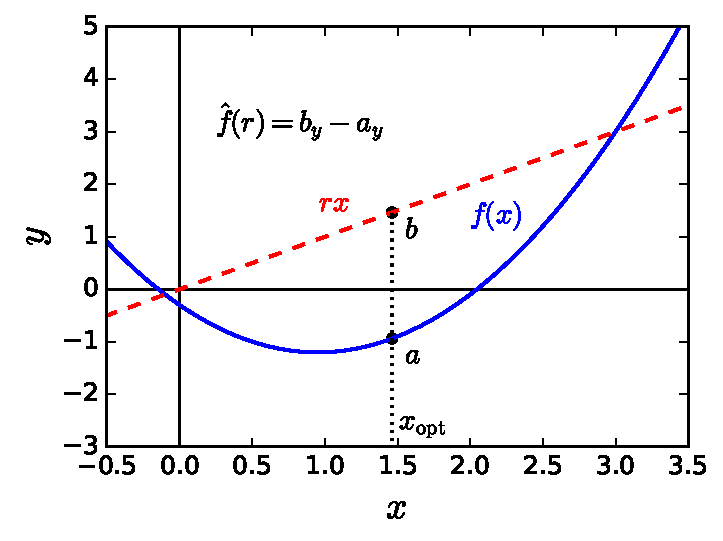
\includegraphics[scale=.65]{img/plots/LT_legendre.pdf}
  \caption[Graphical representation of the Legendre trasnform.]{Graphical representation of the Legendre transform. (blue-line) Convex function, $f(x)=x^2-1.9x-0.3$, to be transformed. (red-dashed) Constant slope line passing by the coordinate system origin, $rx$. The Legendre transform is the maximal difference between $rx$ and $f(x)$ at the same $x$. In this case, the vertical distance between $a$ and $b$.}
  \label{fig:lt-geometric-legendre}
\end{figure}

The inverse transformation is simply obtained by applying again the same technique.
One fully recovers the
\be
  f(x) = \max_{r}\{rx-\hat{f}(r)\}.
\ee

Let us develop the example shown in the Figure~\ref{fig:lt-geometric-legendre}, where the function is $f(x)=x^2-1.9x-0.3$.
In this case the problem is well defined on the complete real axis.
Now, one has to find the maximum of $g(r,x)=rx-f(x)$ for all $r$.
The maximum is easily obtained in this particular case with usual techniques.
On has to solve for x the following equation $\partial_x g(r,x) = 0$. Thus, the maximum is at $x_{\text{opt}} = \frac{r+1.9}{2}$ and hence, the Legendre transform is
\be
  \hat{f}(r) = \frac{r^2}{4}+0.95r+1.2025.
\ee
If one applies again the transformation the resulting function is again the original one.

\subsection{Binomial identities}
\label{app:binomial-identities}

\subsection{Calculation of the QFI matrix elements}
\label{app:matrix-elements-of-QFI}

We start with states insensitive to the homogeneous fields.
Later, we will discuss states sensitive to it.
Next, we must compute the matrix elements of the quantum Fisher information defined for the generators $H_0$ and $H_1$.
We use the functional defined in Eq.~\eqref{eq:gm-FAB} to compute the matrix elements.
We also use thermal states with respect to the spatial degrees of freedom Eq.~\eqref{eq:gm-eigendecomposition-of-state}, since it is one of the most common situations in the experiments.

First of all, we compute the $\mathbfcal{F}_{11}\equiv\qfif{\rho, H_1, H_1}\equiv\qfif{\rho,H_1}$, since it is valid for states that are insensitive to the homogeneous field as well as for states that are sensitive to it.
We have the following for the QFI
\be
\begin{split}
  \qfif{\rho,H_1} &= 2\iint \sum_{\lambda,\nu}\frac{1}{\delta(\bs{0})}
  \frac{(\prob(\bs{x})p_\lambda - \prob(\bs{y})p_\nu)^2}
  {\prob(\bs{x})p_\lambda + \prob(\bs{y})p_\nu}
  |(H_1)_{\bs{x},\lambda;\bs{y},\nu}|^2
  \,\text{d}^N\bs{x} \text{d}^N\bs{y}\\
  &= 2\iint \sum_{\lambda,\nu}\frac{1}{\delta(\bs{0})}
  \frac{(\prob(\bs{x})p_\lambda - \prob(\bs{y})p_\nu)^2}
  {\prob(\bs{x})p_\lambda + \prob(\bs{y})p_\nu}
  (\delta(\bs{x}-\bs{y}))^2\sum_{n,m}^N x_n x_m
  \braopket{\lambda}{j_z^{(n)}}{\nu}\braopket{\nu}{j_z^{(m)}}{\lambda}
  \,\text{d}^N\bs{x} \text{d}^N\bs{y}
\end{split}
\ee
Using the definition of the Dirac delta inside one of the integrals we have that
\be
\begin{split}
  \qfif{\rho,H_1} &= 2\int \sum_{\lambda,\nu}\frac{\prob(\bs{x})}{\delta(\bs{0})}
  \frac{(p_\lambda - p_\nu)^2}
  {p_\lambda + p_\nu}
  \delta(\bs{x}-\bs{x})\sum_{n,m}^N x_n x_m
  \braopket{\lambda}{j_z^{(n)}}{\nu}\braopket{\nu}{j_z^{(m)}}{\lambda}
  \,\text{d}^N\bs{x}\\
  &= 2\int \prob(\bs{x}) \sum_{\lambda,\nu}
  \frac{(p_\lambda - p_\nu)^2}{p_\lambda + p_\nu}
  \sum_{n,m}^N x_n x_m
  \braopket{\lambda}{j_z^{(n)}}{\nu}\braopket{\nu}{j_z^{(m)}}{\lambda}
  \,\text{d}^N\bs{x}\\
  &= \sum_{n,m}^N \int x_n x_m \prob(\bs{x}) \,\text{d}^N\bs{x}\,
  \qfif{\rho_{\text{s}},j_z^{(n)},j_z^{(m)}},
\end{split}
\label{eq:app-computing-f11}
\ee
where we used the Eq.~\eqref{eq:gm-simplify-h1-matrix-els} for the simplification of the matrix elements of $H_1$, where in the third line we used on of the Dirac deltas to eliminate $\bs{y}$ from the equation, and where in the fourth line we toke the $2$ factor in front, the sum over $\lambda$ and $\nu$ and the matrix elements of $j_z^{(n)}$ and $j_z^{(m)}$ and we reconstructed $\qfif{\rho_{\text{s}},j_z^{(n)},j_z^{(m)}}$ using its definition Eq.~\eqref{eq:gm-FAB}.
We finally reordered all the terms in order to group what it has to be integrated together between "$\int$" and "$\text{d}^N\bs{x}$", which in this case represents a two-point correlation function of $x_n$ and $x_m$ over the PDF $\prob(\bs{x})$.

We carry out a similar calculation for $\mathbfcal{F}_{01}$ and $\mathbfcal{F}_{00}$.
We use again a state of the form Eq.~\eqref{eq:gm-eigendecomposition-of-state} to compute these matrix elements of the QFI.
We also use the simplified expression for the matrix elements of $H_0$ for this case Eq.~\eqref{eq:gm-simplify-h0-matrix-els}.
For $\mathbfcal{F}_{01}$, the computation looks like
\be
\begin{split}
  \mathbfcal{F}_{01} &= 2\iint \sum_{\lambda,\nu}\frac{1}{\delta(\bs{0})}
  \frac{(\prob(\bs{x})p_\lambda - \prob(\bs{y})p_\nu)^2}
  {\prob(\bs{x})p_\lambda + \prob(\bs{y})p_\nu}
  (H_0)_{\bs{x},\lambda;\bs{y},\nu}(H_1)_{\bs{y},\nu;\bs{x},\lambda}
  \,\text{d}^N\bs{x} \text{d}^N\bs{y}\\
  &= 2\iint \sum_{\lambda,\nu}\frac{1}{\delta(\bs{0})}
  \frac{(\prob(\bs{x})p_\lambda - \prob(\bs{y})p_\nu)^2}
  {\prob(\bs{x})p_\lambda + \prob(\bs{y})p_\nu}
  (\delta(\bs{x}-\bs{y}))^2\sum_{n,m}^N x_m
  \braopket{\lambda}{j_z^{(n)}}{\nu}\braopket{\nu}{j_z^{(m)}}{\lambda}
  \,\text{d}^N\bs{x} \text{d}^N\bs{y}.
\end{split}
\ee
Using the definition of the Dirac delta inside one of the integrals we have that
\be
\begin{split}
  \mathbfcal{F}_{01} &= 2\int \sum_{\lambda,\nu}\frac{\prob(\bs{x})}{\delta(\bs{0})}
  \frac{(p_\lambda - p_\nu)^2}
  {p_\lambda + p_\nu}
  \delta(\bs{x}-\bs{x})\sum_{n,m}^N x_m
  \braopket{\lambda}{j_z^{(n)}}{\nu}\braopket{\nu}{j_z^{(m)}}{\lambda}
  \,\text{d}^N\bs{x}\\
  &= 2\int \prob(\bs{x}) \sum_{\lambda,\nu}
  \frac{(p_\lambda - p_\nu)^2}{p_\lambda + p_\nu}
  \sum_{n,m}^N x_m
  \braopket{\lambda}{j_z^{(n)}}{\nu}\braopket{\nu}{j_z^{(m)}}{\lambda}
  \,\text{d}^N\bs{x}.
\end{split}
\ee
Which follows from the definition of Eq.~\eqref{eq:gm-FAB}
\be
\begin{split}
  \mathbfcal{F}_{01} &= \sum_{n,m}^N \int x_m \prob(\bs{x}) \,\text{d}^N\bs{x}\,
  \qfif{\rho_{\text{s}},j_z^{(n)},j_z^{(m)}}\\
  &= \sum_{n=1}^N \int x_n \prob(\bs{x}) \,\text{d}^N\bs{x}\,
  \qfif{\rho_{\text{s}},j_z^{(n)},J_z},
\end{split}
\label{eq:app-computing-f01}
\ee
where we used the same arguments as when computing Eq.~\eqref{eq:app-computing-f11}.
We also use the linearity on the second and third arguments of the functional Eq.~\eqref{eq:gm-FAB} in the last line to remove the one of the summation indexes.
Note that the main difference with respect to $\mathbfcal{F}_{11}$ is that in this case the integral represents a single-point average instead of a two-point correlation function.
Finally, for the matrix element $\mathbfcal{F}_{00}$ we have that
\be
\begin{split}
  \mathbfcal{F}_{00} &= 2\iint \sum_{\lambda,\nu}\frac{1}{\delta(\bs{0})}
  \frac{(\prob(\bs{x})p_\lambda - \prob(\bs{y})p_\nu)^2}
  {\prob(\bs{x})p_\lambda + \prob(\bs{y})p_\nu}
  |(H_0)_{\bs{x},\lambda;\bs{y},\nu}|^2
  \,\text{d}^N\bs{x} \text{d}^N\bs{y}\\
  &= 2\iint \sum_{\lambda,\nu}\frac{1}{\delta(\bs{0})}
  \frac{(\prob(\bs{x})p_\lambda - \prob(\bs{y})p_\nu)^2}
  {\prob(\bs{x})p_\lambda + \prob(\bs{y})p_\nu}
  (\delta(\bs{x}-\bs{y}))^2\sum_{n,m}^N
  \braopket{\lambda}{j_z^{(n)}}{\nu}\braopket{\nu}{j_z^{(m)}}{\lambda}
  \,\text{d}^N\bs{x} \text{d}^N\bs{y}.
\end{split}
\ee
We use now the definition of the Dirac delta such that
\be
\begin{split}
  \mathbfcal{F}_{00} &= 2\int \sum_{\lambda,\nu}\frac{\prob(\bs{x})}{\delta(\bs{0})}
  \frac{(p_\lambda - p_\nu)^2}
  {p_\lambda + p_\nu}
  \delta(\bs{x}-\bs{x})\sum_{n,m}^N
  \braopket{\lambda}{j_z^{(n)}}{\nu}\braopket{\nu}{j_z^{(m)}}{\lambda}
  \,\text{d}^N\bs{x}\\
  &= 2\int \prob(\bs{x}) \sum_{\lambda,\nu}
  \frac{(p_\lambda - p_\nu)^2}{p_\lambda + p_\nu}
  \sum_{n,m}^N
  \braopket{\lambda}{j_z^{(n)}}{\nu}\braopket{\nu}{j_z^{(m)}}{\lambda}
  \,\text{d}^N\bs{x}.
\end{split}
\ee
We apply the definition of Eq.~\eqref{eq:gm-FAB} and we reorder terms as
\be
\begin{split}
  \mathbfcal{F}_{00} &= \sum_{n,m}^N \int \prob(\bs{x}) \,\text{d}^N\bs{x}\,
  \qfif{\rho_{\text{s}},j_z^{(n)},j_z^{(m)}}\\
  &= \sum_{n,m}^N \qfif{\rho_{\text{s}},j_z^{(n)},j_z^{(m)}}\\
  &= \qfif{\rho_{\text{s}},J_z,J_z} = \qfif{\rho_{\text{s}},J_z},
\end{split}
\label{eq:app-computing-f00}
\ee
where we simplify the integral using the normalization of the PDF which is equal to $1$.
Note that we obtain the QFI for the homogeneous field as expected.
